%%%%%%%%%%%%%%%%%%%%%%%%%%%%%%%%%%%%%%%%%%%%%%%%%%%%%%%%%%%%%%%%%%%%%%%%
\chapter{Lyra2: a Sponge-based PHS}
%%%%%%%%%%%%%%%%%%%%%%%%%%%%%%%%%%%%%%%%%%%%%%%%%%%%%%%%%%%%%%%%%%%%%%%%
\label{sec:implementation-details}
\label{chapter:lyra2}

This chapter focuses on Lyra2 and its implementation. The cryptographic foundations are outlined in section \ref{sec:lyra2-brief-description}. Section \ref{sec:reference-implementation} describes the architecture of the reference implementation. Finally, section \ref{sec:java-implementation} covers the architecture of the ported implementation as well as a number of challenges that had to be solved.

%=======================================================================
\section{Theoretical Background}
%=======================================================================
\label{sec:lyra2-brief-description}

At the heart of Lyra2 is a \emph{sponge function} or a \emph{sponge construction}. This is an algorithm with finite internal state which takes an input bit stream of arbitrary length and produces an output bit stream of arbitrary length as well \cite{bertoni2007sponge}. The internal state \(S\) consists of \(w = b + c\) bits, where \(w\) is known as the \emph{width} of the sponge, \(b\) is called its \emph{bitrate} and \(c\) its \emph{capacity}. There is a \emph{fixed-width permutation} \(f\) inside of every sponge function. It takes \(w\) bits as input and produces \(w\) bits as output. A common example of \(f\) is Blake2b \cite{aumasson:2013:blake2}, which in its 64-bit modification operates on 128-byte chunks.

As shown in figure \ref{figure:sponge-construction}, a sponge function consists of two stages: the absorbing and the squeezing stage. To start with, an incoming message is padded so that its length is a multiple of \(b\) bits. Next, the internal state of the sponge is initialized with zeros. Then the absorbing phase begins: the next \(b\) bits of the message are XORed with the first \(b\) bits of the state \(S\) and then the permutation \(f\) is applied to the whole \(S\). This process repeats until the entire message has been absorbed. At this point the squeezing phase starts: the first \(b\) bits of \(S\) are emitted and then \(f\) is applied to the whole \(S\). This keeps going until the desired output length is reached.

\begin{figure}
  \begin{tikzpicture}[
  ostyle/.style={
      shape=rectangle
      ,draw
      ,minimum width=0.5cm,
    }
    ,fstyle/.style={
      shape=rectangle
      ,draw
      ,rounded corners=5pt
      ,minimum width=0.5cm
      ,minimum height=5cm
      }
    ,xstyle/.style={
    }
  ]

  \coordinate (A0) at (-0.5, 5) {};
  \coordinate (A1) at (-0.5, 3) {};
  \coordinate (A2) at (-0.5, 0) {};

  \draw [<->,semithick] (A0) to node [left] {\(b\)} (A1);
  \draw [<->,semithick] (A1) to node [left] {\(c\)} (A2);

  \node [ostyle,minimum height=2cm] (00) at (0.5, 4  ) {\(0\)};
  \node [ostyle,minimum height=3cm] (01) at (0.5, 1.5) {\(0\)};

  \node [shape=rectangle,draw] (padded message) at (-0.5, 6) {padded message};

  \coordinate (y0) at (1.5, 6) {};
  \coordinate (y1) at (3.5, 6) {};
  \coordinate (y2) at (5.5, 6) {};
  \coordinate (y3) at (7.5, 6) {};
  \coordinate (y4) at (9.5, 6) {};
  \draw [-] (padded message) to (y0) to (y1) to (y2);

  \node [xstyle] (x0) at (1.5, 4) {\(\oplus\)};
  \node [xstyle] (x1) at (3.5, 4) {\(\oplus\)};
  \node [xstyle] (x2) at (5.5, 4) {\(\oplus\)};
  \coordinate (x3) at (7.5, 4) {};
  \coordinate (x4) at (9.5, 4) {};

  \node [shape=rectangle] (absorb) at (3.5, -1) {absorbing phase};
  \node [shape=rectangle] (squeeze) at (9.5, -1) {squeezing phase};

  \draw [thick,dashed] (7.25, 6.5) -- (7.25, -1.5);

  \draw [->] (y0) to node [right,near start] {1\textsuperscript{st} \(b\) bits} (x0);
  \draw [->] (y1) to node [right,near start] {2\textsuperscript{nd} \(b\) bits} (x1);
  \draw [->] (y2) to node [right,near start] {3\textsuperscript{rd} \(b\) bits} (x2);
  \draw [->] (x3) to node [right,near end] {1\textsuperscript{st} \(b\) bits} (y3);
  \draw [->] (x4) to node [right,near end] {2\textsuperscript{nd} \(b\) bits} (y4);

  \node [fstyle] (f0) at ( 2.5, 2.5) {\(f\)};
  \node [fstyle] (f1) at ( 4.5, 2.5) {\(f\)};
  \node [fstyle] (f2) at ( 6.5, 2.5) {\(f\)};
  \node [fstyle] (f3) at ( 8.5, 2.5) {\(f\)};
  \node [fstyle] (f4) at (10.5, 2.5) {\(f\)};

  \draw [->] (00) to (x0);
  \draw [->] (x0) -- (x0 -| f0.west);
  \draw [->] ($(f0.east) + (0, 1.5)$) -- (x1);
  \draw [->] (x1) -- (x1 -| f1.west);
  \draw [->] ($(f1.east) + (0, 1.5)$) -- (x2);
  \draw [->] (x2) -- (x2 -| f2.west);
  \draw [-] ($(f2.east) + (0, 1.5)$) -- (x3);
  \draw [-] (x3) -- ($(f3.west) + (0, 1.5)$);
  \draw [-] ($(f3.east) + (0, 1.5)$) -- (x4);
  \draw [-] (x4) -- ($(f4.west) + (0, 1.5)$);
  \draw [->] ($(f4.east) + (0, 1.5)$) -- ($(f4.east) + (1, 1.5)$);

  \draw [->] (01) -- (01 -| f0.west);
  \draw [->] ($(f0.east) + (0, -1)$) -- ($(f1.west) + (0, -1)$);
  \draw [->] ($(f1.east) + (0, -1)$) -- ($(f2.west) + (0, -1)$);
  \draw [->] ($(f2.east) + (0, -1)$) -- ($(f3.west) + (0, -1)$);
  \draw [->] ($(f3.east) + (0, -1)$) -- ($(f4.west) + (0, -1)$);
  \draw [->] ($(f4.east) + (0, -1)$) -- ($(f4.east) + (1, -1)$);

  \end{tikzpicture}
  \caption{The sponge construction, adapted from \cite{bertoni:2011:duplexing,marcos:2015:lyra2}}
  \label{figure:sponge-construction}
\end{figure}

A similar cryptographic primitive is the \emph{duplex construction}. The main difference with the sponge construction is that both the absorbtion of incoming bits and the squeezing of the outgoing bits happens simultaneously, in a tick-tock fashion. The name is based on an analogy between the half- and full-duplex modes of communication. A formal description can be found in \cite{bertoni:2011:duplexing} and a visual explanation is provided in figure \ref{figure:duplex-construction}. An important detail is that \cite{bertoni:2011:duplexing} proves that the sponge and the duplex construction are equally secure.

\begin{figure}
  \begin{tikzpicture}[
  ostyle/.style={
      shape=rectangle
      ,draw
      ,minimum width=0.5cm,
    }
    ,fstyle/.style={
      shape=rectangle
      ,draw
      ,rounded corners=5pt
      ,minimum width=0.5cm
      ,minimum height=5cm
      }
    ,xstyle/.style={
    }
  ]

  \coordinate (A0) at (-0.5, 5) {};
  \coordinate (A1) at (-0.5, 3) {};
  \coordinate (A2) at (-0.5, 0) {};

  \draw [<->,semithick] (A0) to node [left] {\(b\)} (A1);
  \draw [<->,semithick] (A1) to node [left] {\(c\)} (A2);

  \node [ostyle,minimum height=2cm] (00) at (0.5, 4  ) {\(0\)};
  \node [ostyle,minimum height=3cm] (01) at (0.5, 1.5) {\(0\)};

  \coordinate (x00) at ( 1.5, 6) {};
  \coordinate (x01) at ( 4.5, 6) {};
  \coordinate (x02) at ( 7.5, 6) {};
  \coordinate (x03) at (10.5, 6) {};

  \node [xstyle] (x10) at ( 1.5, 4) {\(\oplus\)};
  \node [xstyle] (x11) at ( 4.5, 4) {\(\oplus\)};
  \node [xstyle] (x12) at ( 7.5, 4) {\(\oplus\)};
  \node [xstyle] (x13) at (10.5, 4) {\(\oplus\)};

  \draw [->] (x00) to node [anchor=south,rotate=90] {1\textsuperscript{st} \(b\) bits} (x10);
  \draw [->] (x01) to node [anchor=south,rotate=90] {2\textsuperscript{nd} \(b\) bits} (x11);
  \draw [->] (x02) to node [anchor=south,rotate=90] {3\textsuperscript{rd} \(b\) bits} (x12);
  \draw [->] (x03) to node [anchor=south,rotate=90] {4\textsuperscript{th} \(b\) bits} (x13);

  \coordinate (x14) at (13.5, 4) {};
  \coordinate (x24) at (13.5, 1.5) {};

  \coordinate (y00) at (3.5, 6) {};
  \coordinate (y01) at (6.5, 6) {};
  \coordinate (y02) at (9.5, 6) {};

  \coordinate (y10) at (3.5, 4) {};
  \coordinate (y11) at (6.5, 4) {};
  \coordinate (y12) at (9.5, 4) {};

  \draw [<-] (y00) to node [anchor=south,rotate=90] {1\textsuperscript{st} \(b\) bits} (y10);
  \draw [<-] (y01) to node [anchor=south,rotate=90] {2\textsuperscript{nd} \(b\) bits} (y11);
  \draw [<-] (y02) to node [anchor=south,rotate=90] {3\textsuperscript{rd} \(b\) bits} (y12);

  \draw [->] (y10) -- (y00);
  \draw [->] (y11) -- (y01);
  \draw [->] (y12) -- (y02);

  \node [fstyle] (f0) at ( 2.5, 2.5) {\(f\)};
  \node [fstyle] (f1) at ( 5.5, 2.5) {\(f\)};
  \node [fstyle] (f2) at ( 8.5, 2.5) {\(f\)};
  \node [fstyle,dashed] (f3) at (11.5, 2.5) {\(f\)};

  \draw [->] (00) to (x10);
  \draw [->] (x0) -- (x0 -| f0.west);
  \draw [->] ($(f0.east) + (0, 1.5)$) -- (x11);
  \draw [->] (y10) -- (y00);
  \draw [->] (x11) -- (x11 -| f1.west);
  \draw [->] ($(f1.east) + (0, 1.5)$) -- (x12);
  \draw [->] (x12) -- (x12 -| f2.west);
  \draw [->] ($(f2.east) + (0, 1.5)$) -- (x13);
  \draw [->] (x13) -- ($(f3.west) + (0, 1.5)$);
  \draw [->,dashed] ($(f3.east) + (0, 1.5)$) -- (x14);

  \draw [->] (01) -- (01 -| f0.west);
  \draw [->] ($(f0.east) + (0, -1)$) -- ($(f1.west) + (0, -1)$);
  \draw [->] ($(f1.east) + (0, -1)$) -- ($(f2.west) + (0, -1)$);
  \draw [->] ($(f2.east) + (0, -1)$) -- ($(f3.west) + (0, -1)$);
  \draw [->,dashed] ($(f3.east) + (0, -1)$) -- (x24);

  \end{tikzpicture}
  \caption{The duplex construction, adapted from \cite{bertoni:2011:duplexing,marcos:2015:lyra2}}
  \label{figure:duplex-construction}
\end{figure}

The next important component of Lyra2 design is the memory matrix. Its size is directly controlled by the memory cost parameter which corresponds to the number of rows of the matrix. An implementation detail are two other parameters: the number of columns and block length (switches \mintinline{shell}{--blocks} and \mintinline{shell}{--columns} in the lyra2-java project). Their product equals to the number of 64-bit words in a single row of the memory matrix. The reference C implementation sets both of these parameters at compile time while the Java implementation exposes them at runtime.

Conceptually, Lyra2 is an application of a duplex construction which continuously reads and writes blocks to and from the memory matrix. The algorithm is structured into four sequential phases: \emph{Bootstrapping}, \emph{Setup}, \emph{Wandering}, and \emph{Wrap-up}, see figure \ref{fig:basic-structure-lyra2} for reference.

During the \emph{Bootstrapping} phase the main event is the initialization of the sponge. It absorbs the password together with the salt and a few other parameters such as: lengths of output, password and salt, time cost, memory cost and number of columns. If required, this list could be expanded with application-specific information like user- or domain names. An implementation detail is that in case of Blake2b its IVs are used instead of zeroes to initialize part of the sponge state.

The \emph{Setup} phase deals primarily with initializing the memory matrix. The sponge here is used as a duplex construction: it continuously writes to the uninitialized rows of the matrix as well as updates some of the already visited ones. It takes special care so as not to let potential attackers discard parts of the memory matrix. It also speeds up the execution by using a reduced number of rounds of the permutation \(f\). This phase ends once the last row of the matrix is visited.

The \emph{Wandering} phase is the main operation phase of Lyra2. It runs for \(time\_cost \times memory\_cost\) iterations and is by far the longest phase. The fact that both the \(time\_cost\) and the \(memory\_cost\) are decoupled allows legitimate users to fine-tune the parameter values to take full advantage of their platform. During the wandering phase the rows of the memory matrix are continuously revisited and updated in a randomized fashion which is determined by the input parameters. As during the previous phase, special attention is paid to disallow time/memory tradeoffs that would either a) allow to parallelize computations or b) allow to discard parts of the memory matrix and recompute them later.

Finally, the \emph{Wrap-up} phase concludes with a full-round absorbing operation by the sponge (which ensures that Lyra2 is at least as secure as the sponge) and a full-round squeeze operation that produces the requested number of output bits.

For a much more thorough introduction please consult the original paper \cite{andrade:2016:lyra2,marcos:2015:lyra2}.

\begin{figure}[H]
\centering
  \begin{tikzpicture}[phase/.style={rectangle,draw=blue!50,fill=blue!20,thick}]
      \node (phase0) at (0, 0) [phase] {Bootstrapping};
      \node (phase1) [phase,right=of phase0] {Setup};
      \node (phase2) [phase,right=of phase1] {Wandering};
      \node (phase3) [phase,right=of phase2] {Wrap-up};

      \draw [->] (phase0) -- (phase1);
      \draw [->] (phase1) -- (phase2);
      \draw [->] (phase2) -- (phase3);
  \end{tikzpicture}
  \caption{Basic structure of Lyra2. Strictly sequential design.}
  \label{fig:basic-structure-lyra2}
\end{figure}

\section{Reference Implementation}
\label{sec:reference-implementation}

This section will present an overview of relevant parts of the reference implementation. It is hosted as a public GitHub repository \cite{github:2017:lyra}. There are several projects in the same repository (both Lyra2 and Lyra, as well as documentation). The Lyra2 directory of the master branch contains the latest version of the code and documentation. In particular, \path{Lyra2/src} is the root directory for code, \path{Lyra2/src/bench} contains benchmarking shell scripts, \path{Lyra2/src/cuda} contains code that looks how Lyra2 withstands GPU-based attacks, \path{Lyra2/src/sse} contains an sse-optimized implementation. Finally, the \path{Lyra2/src} contains the reference implementation in C99 and is the primary focus of this work.

The original public repository \cite{github:2017:lyra} was forked to \cite{github:2017:lyra-copy} and the following modifications were made. The reference implementation uses \mintinline{shell}{make} as its build system and the \path{Lyra2/src/makefile} provides clear compilation instructions. However, only one version of Lyra2 can be compiled at a time and the provided test vectors are hard-coded into the program. So, the following functionality was added for a more convenient comparison of the reference implementation to its ported Java version:

\begin{itemize}
    \item Compile multiple versions of Lyra2 which could be used simultaneously.
    \item Perform sanity checks of the compiled executable with a set of quick tests.
    \item Compute and store hash values of some test inputs for each version of Lyra2.
  \end{itemize}

This functionality can be found in the \mintinline{shell}{harness} branch of the forked repository \cite{github:2017:lyra-copy} and a pull request \cite{github:2017:lyra-pr} to the reference repository. It is a Python 3 script \mintinline{shell}{Lyra2/tests/harness.py} which can be configured both through the command line and the \mintinline{shell}{Lyra2/tests/harness.yml} configuration file. The \mintinline{shell}{Lyra2/tests/harness.py compile} compiles several Lyra2 reference implementations and the \mintinline{shell}{Lyra2/tests/harness.py compute} runs those implementations on a series of test vectors and records the resulting hash values. Finally, if you install \texttt{py.test} then a call to \texttt{py.test} will run a few unit tests.

\section{Java Implementation}
\label{sec:java-implementation}

It is fair to say that C is primarily a function-based language. At the same time Java is a lot more object-oriented. Therefore, the C functions from the reference implementation need to be translated into (abstract) classes and interfaces of Java. An additional challenge is the fact that the reference implementation uses conditional compilation, so a function with the same name actually contains different code depending on the instructions received by the compiler.

The architecture of the Java project underwent iterative improvements and a reasonably accurate UML diagram of the final version is presented in figure \ref{fig:uml}.


\begin{figure}
\begin{tikzpicture}
    \begin{umlpackage}{lyra2}
        \umlclass{Main}{}{
            \umlstatic{
                + main(argv: String[]): void
            }
        }

        \umlclass[right=1cm of Main]{mem}{}{
            \umlstatic{
                + copy(dst: byte[], offset: int, src: int): void
            } \\
            \umlstatic{
                + flip(x: long): long
            }
        }

        \umlclass[below=0.5cm of Main]{echo}{}{
            \umlstatic{
                + bytes(bytes: byte[], n: int, m: int, s: int): void
            } \\
            \umlstatic{
                + bytes(bytes: byte[], n: int): void
            } \\
            \umlstatic{
                + bytes(longs: long[], n: int, m: int, s: int): void
            } \\
            \umlstatic{
                + bytes(longs: long[], n: int): void
            } \\
            \umlstatic{
                + params(params: LyraParams): void
            }
        }

        \umlclass[right=1cm of echo]{pack}{}{
            \umlstatic{
                + bytes(x: long): byte[]
            } \\
            \umlstatic{
                + bytes(longs: long[]): byte[]
            } \\
            \umlstatic{
                + longs(bytes: byte[]): longs[]
            } \\
            \umlstatic{
                + bytes(strings: String[]): byte[]
            }
        }


        \umlclass[below right=0.5cm and -6cm of echo]{Lyra2}{}
        {
            \umlstatic{
                + phs(hash: byte[], pass: byte[], salt: byte[], params: LyraParams): void
            } \\
            \umlstatic{
                + hash(hash: byte[], pass: byte[], salt: byte[], params: LyraParams): void
            }
        }

        \umlclass[below=0.5cm of Lyra2]{Sponge}{
            + state: long[]
        }{
            + absorb(src: long[], len: int, offset: int): void \\
            + squeeze(dst: byte[], len: int): void \\
            + sponge\_lyra(rounds: int): void \\
            \umlstatic{
                + rotr64(word: long, b: int): void
            } \\
            \umlstatic{
                + rotl64(word: long, b: int): void
            } \\
            \umlvirt{
                + G(a: int, b: int, c: int, d: int): void
            } \\
            + reduced\_squeeze\_row0(dst: long[], offset: int): void \\
            + reduced\_duplex\_row1\_and\_row2(dst: long[], offset1: int, offset2: int): void \\
            + reduced\_duplex\_row\_filling(dst: long[], offset0: int, offset1: int, offset2: int, offset3: int): void \\
            + reduced\_duplex\_row\_wandering(dst: long[], offset0: int, offset1: int, offset2: int, offset3: int): void
        }

        \umlclass[below left=0.5cm and -6cm of Sponge]{SpongeBlake2b}{}{
            + G(a: int, b: int, c: int, d: int): void
        }

        \umlclass[below left=0.5cm and -15cm of Sponge]{SpongeBlamka}{}{
            + G(a: int, b: int, c: int, d: int): void
        }

        \umlclass[below=3cm of Sponge]{SpongeHalfBlamka}{}{
            + G(a: int, b: int, c: int, d: int): void
        }

        \umlHVinherit{SpongeBlake2b}{Sponge}
        \umlHVinherit{SpongeBlamka}{Sponge}
        \umlHVinherit{SpongeHalfBlamka}{Sponge}
      \end{umlpackage}
  \end{tikzpicture}
  \caption{Approximate class diagram for \texttt{com.github.all3fox.lyra2} package}
  \label{fig:uml}
  \end{figure}

The \texttt{Main} class is the entry point of the project. An implementation detail that is not shown in figure \ref{fig:uml} is that the \mintinline{shell}{Main} class relies on a 3\textsuperscript{rd} party command line library \mintinline{shell}{picocli} \cite{web:2017:picocli}. This library parses input parameters (like the password, the salt, etc.) and constructs an instance of the \mintinline{shell}{LyraParams} class. That class is also not shown in figure \ref{fig:uml}, it just stores the parameters and constants relevant to Lyra2's operation. Finally, the \mintinline{shell}{echo} class is a collection of methods for pretty-printing different types of arrays as a table of bytes to the console. Lowercase name of a class is a convention that indicates that this class is a collection of related static methods.

The \mintinline{shell}{mem} and \mintinline{shell}{pack} classes are responsible for memory manipulations. In particular, the \mintinline{java}{mem} class deals with the little- and big-endian discrepancies between the C and Java languages on the \texttt{x86\_64} architecture. The reference implementation is little-endian, which results in bytes being reversed when written to memory, as shown in figure \ref{fig:little-endian}. At the same time the Java virtual machine is big-endian. This is why the \mintinline{java}{long mem.flip(long x)} method is used constantly to reverse bytes back and forth in lyra2-java.

The \mintinline{java}{pack} class provides methods that allow to partially emulate the pointer casting which happens in C. It is often the case in C that a chunk of memory is allocated and treated as individual bytes or some larger data type, like \mintinline{c}{uint64_t}. The C language allows to cast a \mintinline{c}{void*} pointer to \mintinline{c}{char*} or \mintinline{c}{uint64_t*}, depending on the situation. This also affects array indexing because the perceived size of the underlying element changes event though the bytes themselves remain the same. In other words, depending on the type of the pointer, a \mintinline{c}{*(ptr1 + 5)} might be the beginning of the same element as \mintinline{c}{*(ptr2 + 1)}.

In order to circumvent this, the \mintinline{java}{pack} class provides a number of overloaded methods, where \mintinline{java}{pack.bytes(long[] xs)} takes \texttt{xs} and returns a copy of the same data in an array of type \mintinline{java}{byte} and \mintinline{java}{pack.longs(byte[] xs)} does the reverse for \mintinline{java}{long}. Of course, this introduces an expensive array copy. This copy does not happen during \emph{Setup} and \emph{Wandering} phases.

\begin{figure}
    \centering
    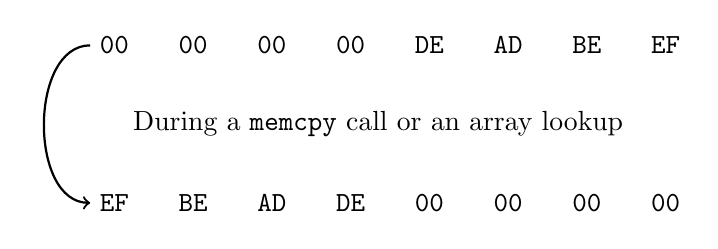
\begin{tikzpicture}
        \node (0)              {\texttt{00}};
        \node (1) [right of=0] {\texttt{00}};
        \node (2) [right of=1] {\texttt{00}};
        \node (3) [right of=2] {\texttt{00}};
        \node (4) [right of=3] {\texttt{DE}};
        \node (5) [right of=4] {\texttt{AD}};
        \node (6) [right of=5] {\texttt{BE}};
        \node (7) [right of=6] {\texttt{EF}};

        \node (H0) [below of=0] {};

        \node (A) [below of=H0]  {\texttt{EF}};
        \node (B) [right of=A] {\texttt{BE}};
        \node (C) [right of=B] {\texttt{AD}};
        \node (D) [right of=C] {\texttt{DE}};
        \node (E) [right of=D] {\texttt{00}};
        \node (F) [right of=E] {\texttt{00}};
        \node (G) [right of=F] {\texttt{00}};
        \node (H) [right of=G] {\texttt{00}};

        \draw [thick,out=180,in=180,->] (0) to node [right=1cm] {During a \texttt{memcpy} call or an array lookup} (A);
      \end{tikzpicture}
    \caption{The byte swap on a little-endian platform (i.e. C99 on \texttt{x86\_64})}
    \label{fig:little-endian}
  \end{figure}

The \mintinline{java}{Lyra2} class contains the main logic of the single-threaded Lyra2 instance. The functionality related to the sponge construction is captured by the \mintinline{java}{Sponge} \emph{abstract} class. Its subclasses \mintinline{java}{SpongeBlake2b}, \mintinline{java}{SpongeBlamka} and \mintinline{java}{SpongeHalfBlamka} hold the specifics of the underlying fixed-width permutation \(f\).

An interesting detail is that the Sponge class in the Java project makes use of both left- and right bit rotations, done by the \texttt{rotl64} and \texttt{rotr64} methods respectively. These methods accept a 64 bit \mintinline{java}{long} and rotates it by the specified number of bits \mintinline{java}{b}. Those rotations are \emph{not} arithmetic and do \emph{not} preserve the sign of their argument.

The original Lyra2 reference implementation requires just one direction for rotations. Both types of rotations are helpful in lyra2-java because they allow to avoid a number of byte rotations related to endianness. For an example of this,  refer to figure \ref{fig:sponge-blake2b}. It shows the \texttt{SpongeBlake2b} implementation, where lines \(5, 8\), and \(11\) use a left rotation. The original Blake2b specification prescribes a right rotation for those steps. However, instead of calling \mintinline{java}{mem.flip} that would rotate its argument once and then actually rotate it with \mintinline{java}{Sponge.rotr64}, a single rotation in the other direction with \mintinline{java}{Sponge.rotl64} is performed.

The same trick cannot be performed on line \(16\) though. The rotation there is \(63\) bits to the right, which is not divisible by 8 bits (the size of one byte). Since \mintinline{java}{mem.flip} performs a byte-level rotation, it does not mix with the rotation and has to be performed explicitly. This rotation trick has accelerated the ported implementation by about 20\%. The BlaMka family of sponges are based on Blake2b and benefit from the same trick as well, see figure \ref{fig:sponge-blamka}.

\begin{figure}
\small
\begin{minted}[linenos]{java}
    public class SpongeBlake2b extends Sponge {
        @Override
        public void G(final int a, final int b, final int c, final int d) {
            state[a] = mem.flip(mem.flip(state[a]) + mem.flip(state[b]));
            state[d] = rotl64(state[d] ^ state[a], 32);

            state[c] = mem.flip(mem.flip(state[c]) + mem.flip(state[d]));
            state[b] = rotl64(state[b] ^ state[c], 24);

            state[a] = mem.flip(mem.flip(state[a]) + mem.flip(state[b]));
            state[d] = rotl64(state[d] ^ state[a], 16);

            state[c] = mem.flip(mem.flip(state[c]) + mem.flip(state[d]));
            // Cannot use the left rotation trick here: 63 % 8 != 0, so
            // individual bytes do not stay the same, they change too.
            state[b] = mem.flip(rotr64(mem.flip(state[b] ^ state[c]), 63));
        }
    }
\end{minted}
\normalsize
\caption{Blake2b as instance of the Sponge class, demonstrating optimized rotations on lines 5, 8 and 11. Line 16 performs the complete set of rotations (no optimization).}
\label{fig:sponge-blake2b}
\end{figure}


\begin{figure}
\small
\begin{minted}[linenos]{java}
public class SpongeBlamka extends Sponge {
    private long fBlaMka(final long x, final long y) {
        long lessX = 0x00000000FFFFFFFFL & x;
        long lessY = 0x00000000FFFFFFFFL & y;

        lessX *= lessY;

        lessX <<= 1;

        return lessX + x + y;
    }

    @Override
    public void G(final int a, final int b, final int c, final int d) {
        state[a] = mem.flip(fBlaMka(mem.flip(state[a]), mem.flip(state[b])));
        state[d] = rotl64(state[d] ^ state[a], 32);

        state[c] = mem.flip(fBlaMka(mem.flip(state[c]), mem.flip(state[d])));
        state[b] = rotl64(state[b] ^ state[c], 24);

        state[a] = mem.flip(fBlaMka(mem.flip(state[a]), mem.flip(state[b])));
        state[d] = rotl64(state[d] ^ state[a], 16);

        state[c] = mem.flip(fBlaMka(mem.flip(state[c]), mem.flip(state[d])));
        // Cannot use the left rotation trick here: 63 % 8 != 0, so
        // individual bytes do not stay the same, they change too.
        state[b] = mem.flip(rotr64(mem.flip(state[b] ^ state[c]), 63));
    }
}
\end{minted}
\normalsize
\caption{BlaMka as instance of the Sponge class, the same rotation trick in action on lines 16, 19 and 22. Line 27 performs the complete set of rotations (no optimization).}
\label{fig:sponge-blamka}
\end{figure}
